\documentclass[12pt]{article}

\usepackage{fullpage}
\usepackage[spanish]{babel}
\usepackage{amsfonts} %for double trace letters
\usepackage{amssymb}
\usepackage{amsmath} %for special/unusual mathematical characters
\usepackage{eufrak} %for gothic letters
\usepackage{graphicx} %Image includer package
\graphicspath{{Images/}} %Image directory
\usepackage{xcolor}
\usepackage{esint} % for simple counter-clockwise directed contour integral symbol

\usepackage{multicol} %For writing text in columns
\setlength{\columnsep}{1cm} %Defines separation of columns

\usepackage{tcolorbox} %for boxes that enclose text
\usepackage{color}
\definecolor{myblue}{rgb}{.8, .8, 1}

\usepackage{empheq}

%for green eq box
%\definecolor{lightgreen}{HTML}{90EE90}
%\newcommand{\boxedeq}[2]{\begin{empheq}[box=\colorbox{lightgreen}]{align}\label{#1}#2\end{empheq}}

%for blue eq box
\newlength\mytemplen
\newsavebox\mytempbox

\makeatletter
\newcommand\mybluebox{%
    \@ifnextchar[%]
       {\@mybluebox}%
       {\@mybluebox[0pt]}}

\def\@mybluebox[#1]{%
    \@ifnextchar[%]
       {\@@mybluebox[#1]}%
       {\@@mybluebox[#1][0pt]}}

\def\@@mybluebox[#1][#2]#3{
    \sbox\mytempbox{#3}%
    \mytemplen\ht\mytempbox
    \advance\mytemplen #1\relax
    \ht\mytempbox\mytemplen
    \mytemplen\dp\mytempbox
    \advance\mytemplen #2\relax
    \dp\mytempbox\mytemplen
    \colorbox{myblue}{\hspace{1em}\usebox{\mytempbox}\hspace{1em}}}

% for theorems
\usepackage{amsthm}
 
\theoremstyle{definition}
\newtheorem{definition}{Definici\'on}[section]

\theoremstyle{theorem}
\newtheorem{theorem}{Teorema}[section]

\theoremstyle{corolary}
\newtheorem{corolary}{Corolario}[section]

\DeclareMathOperator{\Arg}{Arg}
\DeclareMathOperator{\Log}{Log}
\DeclareMathOperator{\sen}{sen}
\DeclareMathOperator{\senh}{senh}
\DeclareMathOperator{\tg}{tg}
\DeclareMathOperator{\ctg}{ctg}
\DeclareMathOperator{\tgh}{tgh}
\DeclareMathOperator{\ctgh}{ctgh}
\DeclareMathOperator{\sech}{sech}
\DeclareMathOperator{\csch}{csch}


\begin{document}

	\title{Integraci\'on Compleja}
	\author{Breggia, Bruno M.}
	\date{}
	\maketitle

\begin{center}
	
\includegraphics[scale=0.7]{camino_amarillo.jpg}\\
	\textit{``Sigue el camino amarillo"}\\ - El Mago de Oz -
\end{center}

Sabemos derivar funciones complejas, gran haza\~na. ?`Qu\'e toca ahora? Saber integrarlas. Y para ello contamos con varias herramientas que nos simplificar\'an esta tarea, herramientas que aprenderemos en este cap\'itulo, y provistas la mayor\'ia por un simp\'atico matem\'atico llamado \textit{Augustin Louis Cauchy}, hombre que dej\'o su nombre escrito por todos los libros de c\'alculo complejo (ya hemos visto su nombre antes, ?`recuerdan?). Integrar funciones de variable compleja no se compara tanto con integrar funciones de una variable real, sino con funciones multivariables. Sigue el camino y encontrar\'as la verdad.

\pagebreak
\tableofcontents
\pagebreak

\section{Integral de Funci\'on Compleja con Variable Real}

Avanzaremos por pasos, pues el aprendizaje es procedural y todo tiene un orden que ser seguido para entender conceptos de complejidad creciente. Veremos primero c\'omo integrar funciones que mapean n\'umeros reales con n\'umeros complejos, es decir, funciones complejas \textbf{de variable real}. No se confundan que a diferencia de las funciones que se ven\'ian viendo hasta ahora, \'estas reciben s\'olo un real $t \in \mathbb{R}$ y retornan un complejo, no reciben un complejo, como las t\'ipicas \textbf{funciones de variable compleja}.

Las funciones complejas de variable real mapean puntos en la recta num\'erica $\mathbb{R}$ a puntos en el plano $\mathbb{C}$. Bajo este punto de vista, conviene confesar que describen trayectorias en el plano, son \textit{parametrizaciones}.

Ahora estamos listos para definir la integral de este tipo de funciones:\\

\colorbox{orange!40!white!80}{\parbox{\linewidth}{
 \theoremstyle{definition}
 \begin{definition}{Integral definida de funciones complejas de variable real}

  	T\'engase $$w:\: I=[a, b] \subset \mathbb{R} \rightarrow \mathbb{C}$$donde $w(t) = u(t)+i\ v(t), t\in I$ en el cual $u, v :\: t\in[a, b] \rightarrow \mathbb{R}$\\
  	La \textbf{integral definida} de $w(t)$ sobre $[a,b]$ se simboliza como $\int\limits_a^b w(t)\ dt$ y se define como:
  	$$\int\limits_a^b w(t)\ dt \triangleq \int\limits_a^b u(t)\ dt + i\ \int\limits_a^b v(t)\ dt$$
  	s\'olo en caso de que $\int_a^b u(t)\ dt$ y $\int_a^b v(t)\ dt$ existan.
 \end{definition}}}
\linebreak
\linebreak

Con esta definic\'on, volvemos a la tendencia de definir operaciones sobre complejos en t\'erminos de la misma operaci\'on aplicada a los n\'umeros reales, que ya sabemos c\'omo operan. Esto nos ayuda a simplificar un mont\'on el operar con complejos. Si sabes integrar funciones reales de variable real, sabes integrar funciones complejas de variable real, pues en fin, estar\'as integrando las funciones componentes de la funci\'on compleja, y \'estas no son m\'as que funciones reales.

De igual manera, se pueden definir las integrales impropias de $w(t)$ sobre intervalos no acotados.\\

\colorbox{orange!40!white!80}{\parbox{\linewidth}{
\theoremstyle{theorem}
\begin{definition} {Integrabilidad}

Una funci\'on compleja de variable real diremos que es \textbf{integrable} si sus funciones componentes son continuas \'o presentan una cantidad finita de discontinuidades de salto finito.

\end{definition}}}
\linebreak
\linebreak

Como notamos, las condiciones de integrabilidad son las mismas que para funciones reales. Por ahora, absolutamente nada distinto...	

Ahora, un detalle no menor, la integral definida de funciones complejas de variables real es en s\'i mismo un n\'umero complejo. Simb\'olicamente, $$\int_a^bw(t)\ dt \in \mathbb{C}$$
a partir de cuya definici\'on tenemos que:

$$ \mathfrak{Re}\left[ \int_a^bw(t)\ dt \right] = \int_a^b\mathfrak{Re}[w(t)]\ dt$$
$$ \mathfrak{Im}\left[ \int_a^bw(t)\ dt \right] = \int_a^b\mathfrak{Im}[w(t)]\ dt$$
\linebreak
Ahora estudiaremos algunas propiedades importantes de la integral definida de funciones complejas de variable real. Sean $w, w_1, w_2:\: I=[a,b]\subset \mathbb{R} \rightarrow \mathbb{C}$, y si existen las integrales
$\int_a^bw(t)\ dt, \int_a^bw_1(t)\ dt$ y $\int_a^bw_2(t)\ dt$,
entonces se cumplen:
\begin{enumerate}
	\item Linealidad
	\begin{empheq}[box={\mybluebox[5pt]}]{equation*}
		\mbox{ \large $\int\limits_a^b z_0w(t)\ dt = z_0 \int\limits_a^bw(t)\ dt,\qquad z_0 \in \mathbb{C}$}
	\end{empheq}
	
	\begin{empheq}[box={\mybluebox[5pt]}]{equation*}
		\mbox{ \large $\int\limits_a^b [w_1(t) \pm w_2(t)]\ dt = \int\limits_a^b w_1(t)\ dt \pm \int\limits_a^b w_2(t)\ dt$}
	\end{empheq}
			
	\item Inversi\'on de los extremos de integraci\'on
	\begin{empheq}[box={\mybluebox[5pt]}]{equation*}
		\mbox{ \large $\int\limits_a^b w(t)\ dt = -\int\limits_b^a w(t)\ dt$}
	\end{empheq}
	
	\item Igualdad de los extremos de integraci\'on
	\begin{empheq}[box={\mybluebox[5pt]}]{equation*}
		\mbox{ \large $\int\limits_a^a w(t)\ dt = 0$}
	\end{empheq}
	
	\item Aditividad del intervalo
	\begin{empheq}[box={\mybluebox[5pt]}]{equation*}
		\mbox{ \large $\int\limits_a^c w(t)\ dt = \int\limits_a^b w(t)\ dt + \int\limits_b^c w(t)\ dt, \qquad a<b<c$}
	\end{empheq}
	
	\item Acotaci\'on del m\'odulo
	\begin{empheq}[box={\mybluebox[5pt]}]{equation*}
		\mbox{ \large $ \left| \int\limits_a^b w(t)\ dt \right| \leq \int\limits_a^b |w(t)|\ dt, \qquad a\leq b$}
	\end{empheq}
	
	//Demostrar todas
	
\end{enumerate}

\subsection{Teorema Fundamental del C\'alculo}
Muy linda la definici\'on de integral definida, pero... para resolverla num\'ericamente necesitamos valernos sin lugar a dudas del famoso \textbf{Teorema Fundamental del C\'alculo}. Lo aplicamos porque la integral de funciones complejas de variable real se reduce a integrales de funciones reales, pero la definici\'on misma nos permite extender el teorema para que tenga validez de igual manera por sobre el conjunto de las funciones complejas.\\

\colorbox{magenta!40!white!80}{\parbox{\linewidth}{
\theoremstyle{theorem}
\begin{theorem} {TFC para funciones complejas}

Sea $w:I = [a,b]\subset \mathbb{R}\rightarrow \mathbb{C}$, con $w(t) = u(t) + i\ v(t)$ continua sobre $I$ y $W'(t) = w(t)\ \forall t\in (a, b)$. Entonces:

$$\int_a^b w(t)\ dt = W(b) - W(a) $$

\end{theorem}}}
\linebreak
\linebreak

Considerando $U(t)$ y $V(t)$ primitivas de $u(t)$ y $v(t)$ respectivamente, para $a\leq t \leq b$, entonces $U'(t) = u(t), V'(t) = v(t)$ y podemos expresar la integral definida como:
\begin{eqnarray*}
\int_a^b w(t)\ dt &=& W(b) - W(a)\\
\int_a^b w(t)\ dt &=& [U(b)-U(a)] + i\ [V(b)-V(a)]
\end{eqnarray*}

Siendo que $W(t) = U(t)+i\ V(t)$

\section{Curvas en el plano de Argand}
Volvemos a concebir al plano complejo como ente geom\'etrico para introducir unas nuevas definiciones, que en su momento no se dieron ya que ir\'ian a ser temas dejados de lado hasta este preciso momento. Nos referiremos primero a \textit{parametrizaciones} en el plano complejo, es decir, a aquellas curvas en el plano $\mathbb{C}$ dadas por funciones complejas de variable real. O sea, dependiente de un \textit{par\'ametro} $t \in \mathbb{R}$.

Con esto tenemos como prop\'osito dar a conocer las posibles trayectorias a partir de las cuales pretendemos integrar.

Antes de empezar a tirar definiciones, aclaramos que las mismas se har\'an respecto a una curva $\mathcal{C}: z = z(t)$, con $z:\:I=[a, b]\subset \mathbb{R} \rightarrow \mathbb{C}$, donde $z(t) = x(t)+i\ y(t)$ y: $$x:\ I=[a,b] \subset \mathbb{R} \rightarrow \mathbb{R}$$ $$y:\ I=[a,b] \subset \mathbb{R} \rightarrow \mathbb{R}$$
\linebreak

\colorbox{orange!40!white!80}{\parbox{\linewidth}{
 \theoremstyle{definition}
 \begin{definition}{Arco}

Sean $x=x(t)$ y $y=y(t)$ funciones reales continuas de par\'ametro real $t\in I = [a, b]$. Entonces el conjunto de puntos $\mathcal{C} = \{ z(t)\ /\ z(t)=x(t)+i\ y(t)\}$ es un \textbf{arco}.  	
 \end{definition}}}
\linebreak
\linebreak

\colorbox{orange!40!white!80}{\parbox{\linewidth}{
\theoremstyle{definition}
\begin{definition}{Arco Simple o Arco de Jordan}

Un arco $\mathcal{C}: z(t)$ con $t\in I = [a,b]$ es un \textbf{arco simple} o \textbf{arco de Jordan} si no tiene intersecci\'on consigo mismo, esto es, si se cumple que $z(t_1)\neq z(t_2)$ siempre que $t_1\neq t_2$.\\

En otras palabras, $\mathcal{C}$ es un arco simple si $z(t)$ es inyectiva en el intervalo $I$.
\end{definition}}}
\linebreak
\linebreak

\colorbox{orange!40!white!80}{\parbox{\linewidth}{
\theoremstyle{definition}
\begin{definition}{Arco Diferenciable}

Un arco $\mathcal{C}: z(t)$ con $t\in I = [a,b]$ es un \textbf{arco diferenciable} si $z(t)$ tiene derivada primera continua sobre $I$. En este caso, la funci\'on $$|z'(t)| = \sqrt{[x'(t)]^2+[y'(t)]^2}$$ es integrable en el intervalo $[a, b]$ y la longitud de $\mathcal{C}$ est\'a dada por $L=\int_a^b|z'(t)|\ dt$.
\end{definition}}}
\linebreak
\linebreak

\colorbox{orange!40!white!80}{\parbox{\linewidth}{
\theoremstyle{definition}
\begin{definition}{Arco Suave}

Un arco se dice ser un \textbf{arco suave} si es un arco simple, diferenciable y con $z'(t)\neq 0$ $\forall t \in (a, b)$.\\

Se define para este caso el \textbf{vector tangente unitario}: $$T = \frac{z'(t)}{|z'(t)|}\ \qquad \forall t \in (a,b)$$ cuyo \'angulo de inclinaci\'on es $\phi = \arg z'(t)$.
\end{definition}}}
\linebreak
\linebreak

\colorbox{orange!40!white!80}{\parbox{\linewidth}{
\theoremstyle{definition}
\begin{definition}{Contorno o Camino (o Arco suave por tramos)}

Llamaremos a $\mathcal{C}$ un \textbf{contorno}, \textbf{camino} o inclusive \textbf{arco suave por tramos} si:
\begin{enumerate}
	\item $\mathcal{C} = \bigcup\limits_{k=1}^K \mathcal{C}_k\ /\ \mathcal{C}_k:z = z_k(t)$, en donde $z_k(t)$ es un arco suave en $t\in I_k = [t_{k-1}, t_k]$ con $k=1, 2, ..., K$ y $\bigcup\limits_{k=1}^K I_k = [a, b]$ 
	\item $z(t)$ es continua en $t_k$ con $k=1, 2,..., K-1$
	\item $z'(t)$ puede tener un punto de discontinuidad de salto finito en $t_k$ con $k=1, 2,..., K-1$
\end{enumerate}
\end{definition}}}
\linebreak
\linebreak

\begin{center}
	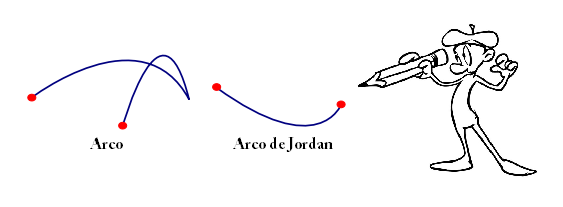
\includegraphics[scale=1]{curva2.png}
\end{center}

\colorbox{orange!40!white!80}{\parbox{\linewidth}{
\theoremstyle{definition}
\begin{definition}{Curva Cerrada Simple}

Llamaremos \textbf{curva cerrada simple} a un arco tal que $z=z(t)$ es inyectiva en $(a, b\ ]$ y que $z(a)=z(b)\:\land\:z'(a)=z'(b)$.
\end{definition}}}
\linebreak
\linebreak

\colorbox{orange!40!white!80}{\parbox{\linewidth}{
\theoremstyle{definition}
\begin{definition}{Curva Cerrada Suave}

Llamaremos \textbf{curva cerrada suave} a la curva $\mathcal{C}: z=z(t)$ en $t\in I = [a,b]$ que satisface:
\begin{enumerate}
	\item $z(t)$ es diferenciable
	\item $z(t)$ es inyectiva sobre $(a, b\ ]$, es decir no se corta a s\'i misma
	\item $z'(t)\neq 0$ adem\'as de que $z(a)=z(b)\:\land\:z'(a)=z'(b)$
\end{enumerate}
\end{definition}}}
\linebreak
\linebreak

\colorbox{orange!40!white!80}{\parbox{\linewidth}{
\theoremstyle{definition}
\begin{definition}{Contorno o Camino cerrado simple}

Llamaremos \textbf{contorno cerrado simple} o \textbf{camino cerrado simple} a la curva $\mathcal{C}: z=z(t)$ en $t\in I = [a,b]$ que satisface:
\begin{enumerate}
	\item $\mathcal{C} = \bigcup\limits_{k=1}^K \mathcal{C}_k\ /\ \mathcal{C}_k:z = z_k(t)$, en donde $z_k(t)$ es un arco suave en $t\in I_k = [t_{k-1}, t_k]$ con $k=1, 2, ..., K$ y $\bigcup\limits_{k=1}^K I_k = [a, b]$ 
	\item $z(t)$ es continua en $t_k$ con $k=1, 2,..., K-1$
	\item $z'(t)$ puede tener un punto de discontinuidad de salto finito en $t_k$ con $k=1, 2,..., K-1$
	\item $z=z(t)$ es inyectiva sobre $(a, b\ ]$ y satisface que $z(a)=z(b)$ y que $z'(a)=z'(b)$.
\end{enumerate}
\end{definition}}}
\linebreak

\begin{center}
	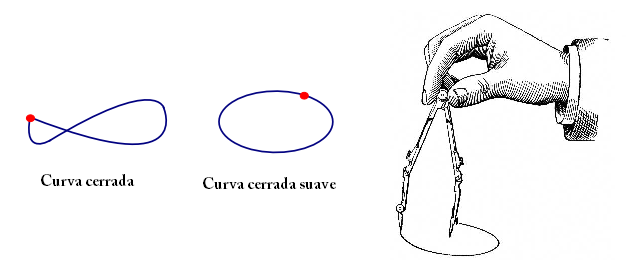
\includegraphics[scale=1]{curva3.png}
\end{center}

Ahora veremos una clasificaci\'on m\'as para dominios en el plano complejo. Se ha visto antes que un dominio es \textbf{conexo} si cualquier par de puntos en \'el se pueden unir mediante una poligonal tal que ning\'un segmento de la misma pase por puntos por fuera del dominio. Con esto en mente, daremos cuenta de una subclasificaci\'on de la \textit{conexidad}.\\

\colorbox{orange!40!white!80}{\parbox{\linewidth}{
\theoremstyle{definition}
\begin{definition}{Dominio Simplemente y M\'ultiplemente Conexo}

Se dice que $\mathcal{D}$ es un dominio \textbf{simplemente conexo} si todo contorno cerrado simple contenido en \'el encierra s\'olo puntos de $\mathcal{D}$.

Si $\mathcal{D}$ no es simplemente conexo, se dice ser \textbf{m\'ultiplemente conexo}.
\end{definition}}}
\linebreak
\linebreak

\begin{center}
	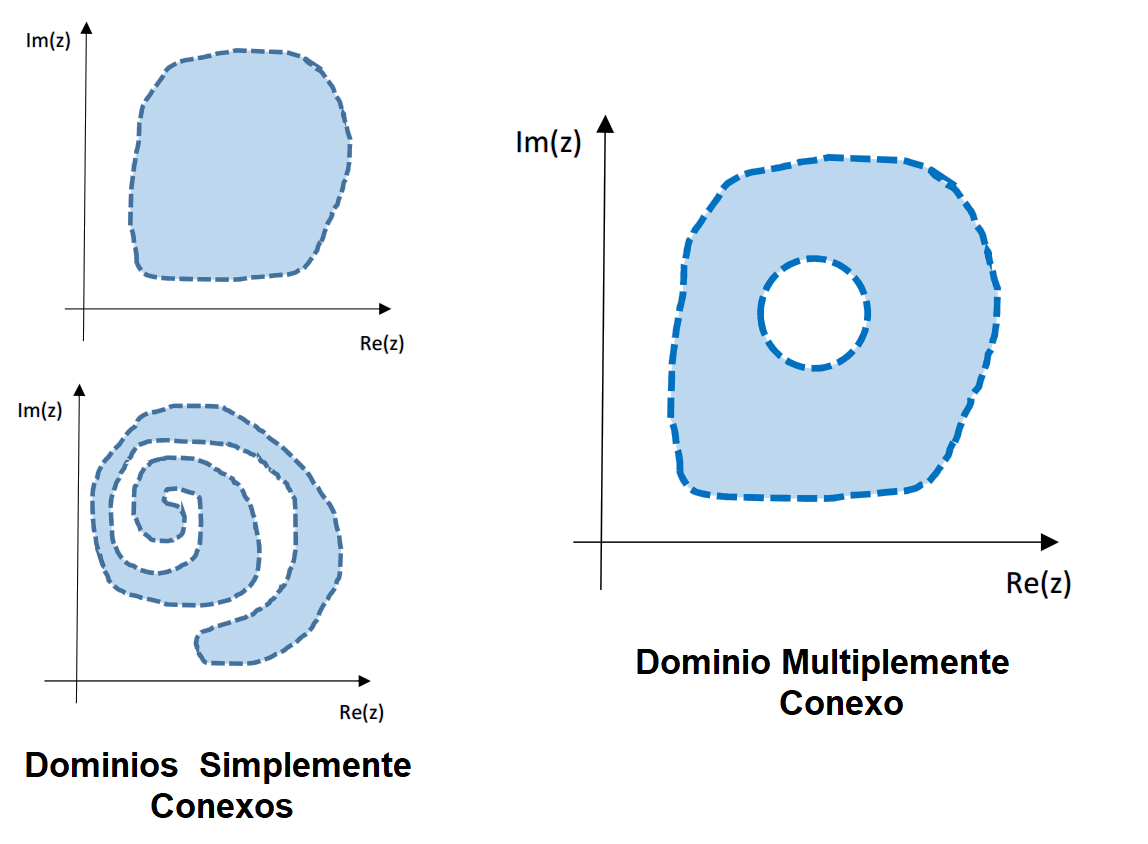
\includegraphics[scale=0.5]{dominios.png}
\end{center}

\section{Integrales de Camino}
Lleg\'o el momento... de integrar funciones complejas de variable compleja. No tengan p\'anico, que es similar a algo que ya conocemos: integrar funciones de varias variables. Si asociamos el plano complejo $\mathbb{C}$ una vez m\'as con $\mathbb{R}^2$, entonces vamos a poder integrar siguiendo trayectorias, curvas, por sobre el plano complejo. Esto quiere decir que siempre que integremos una funci\'on compleja de variable compleja, lo haremos a lo largo de una trayectoria. Como que no tiene sentido si no... e integrar por sobre una trayectoria implica parametrizar el camino que se quiere seguir, o por lo menos, si es que quieres llegar a resolver num\'ericamente la integral (!`c\'omo no resolverla!).

Por ello mismo, a las integrales definidas de funciones complejas de variable compleja las denominaremos \textit{integrales de camino}.\\

\colorbox{green!40!white!80}{\parbox{\linewidth}{
 \theoremstyle{definition}
 \begin{definition}{Integral de Camino o de Contorno}\\

  	Sea un camino $\mathcal{C}: z = z(t) $, donde $z: t\in I =[a, b]\subset \mathbb{R} \rightarrow z(t) \in \mathcal{D}\subset \mathbb{C}_z$ con $z(t) = x(t)+i\ y(t)$ y $z'(t) = x'(t)+i\ y'(t)$ siendo $z'(t)$ continua a trozos sobre $I$.\\
  	
  	Sea $f:z\in \mathcal{C} \rightarrow f(z)\in \mathbb{C}_w$, con $f(z) = u(x, y)+i\ v(x, y)$ definida y continua a trozos sobre $\mathcal{C}$, es decir $f(z(t))$ definida y seccionalmente continua sobre $I=[a,b]$.\\
  	
  	Se define la \textbf{integral de camino}, o \textbf{integral de contorno}, de $f$ a lo largo de $\mathcal{C}$, que se denota $\int_{\mathcal{C}}f(z)\ dz$, como: $$\int\limits_{\mathcal{C}}f(z)\ dz \triangleq \int\limits_a^bf(z(t))\ z'(t)\ dt$$
  	
 \end{definition}}}
\linebreak
\linebreak

Claramente notar\'an que a la integral de contorno la definimos tras el tel\'on en t\'erminos de la integral anteriormente presentada, es decir, de la integral de funciones complejas de variable \textit{real}.

Daremos cuenta ahora, como corresponde a la rutina, de las propiedades con las que cumple este tipo de integral. Si existen $\int_{\mathcal{C}}f(z)\ dz$, $\int_{\mathcal{C}}f_1(z)\ dz$ y $\int_{\mathcal{C}}f_2(z)\ dz$, entonces se cumple:
\begin{enumerate}
	\item Linealidad
	\begin{empheq}[box={\mybluebox[5pt]}]{equation*}
		\mbox{ \large $\int\limits_{\mathcal{C}} z_0f(z)\ dz = z_0 \int\limits_{\mathcal{C}}f(z)\ dz,\qquad z_0 \in \mathbb{C}$}
	\end{empheq}
	
	\begin{empheq}[box={\mybluebox[5pt]}]{equation*}
		\mbox{ \large $\int\limits_{\mathcal{C}} [f_1(z)\pm f_2(z)]\ dz = \int\limits_{\mathcal{C}}f_1(z)\ dz \pm \int\limits_{\mathcal{C}}f_2(z)\ dz$}
	\end{empheq}
	
	\item Inversi\'on de la Orientaci\'on
	\begin{empheq}[box={\mybluebox[5pt]}]{equation*}
		\mbox{ \large $\int\limits_{\mathcal{C}} f(z)\ dz =- \int\limits_{-\mathcal{C}} f(z)\ dz$}
	\end{empheq}
	
	\item Concatenaci\'on de $\mathcal{C}_k$\\
	Sea $\mathcal{C}=\bigcup\limits_{k=1}^{K}\mathcal{C}_k = \mathcal{C}_1 \cup \mathcal{C}_2 \cup\ ...\ \mathcal{C}_K$, con $\mathcal{C}_k$ un contorno en $\mathbb{C}$.

	\begin{empheq}[box={\mybluebox[5pt]}]{equation*}
		\mbox{ \large $\int\limits_{\mathcal{C}}f(z)\ dz = \sum\limits_{k=1}^N \left(\int\limits_{\mathcal{C}_k} f(z)\ dz \right)$}
	\end{empheq}
	
	\item Desigualdad ML\\
	Sea $f(z)$ continua a trozos sobre $\mathcal{C}$ y $|f(z)| \leq M\; \forall z\in \mathbb{C}$.\\
	Sea $L$ la longitud del contorno $\mathcal{C}$.
	
	\begin{empheq}[box={\mybluebox[5pt]}]{equation*}
		\mbox{ \large $\left|\int\limits_{\mathcal{C}}f(z)\ dz \right| \leq ML$}
	\end{empheq}
	
	Demostrar todos
	
\end{enumerate}

\subsection{Relaci\'on con la Integral de L\'inea de funciones reales}
La integral de camino se relaciona sin lugar a dudas con la conocida integral de l\'inea para funciones reales. Pero a no confundirse: \textbf{integral de camino} (para funciones de variable compleja) con \textbf{integrales de l\'inea} (para funciones de variable real). Sin embargo podemos expresar la de contorno en t\'erminos directamente de la de l\'inea, partiendo de su definici\'on:

Sea un contorno $\mathcal{C}: z = z(t)$ con $z: t\in I=[a,b]\subset \mathbb{R}\rightarrow \mathcal{D}\subset \mathbb{C}_z$ donde $z(t)=x(t)+i\ y(t)$ y $z'(t) = x'(t) + i\ y'(t)$. Sea tambi\'en $f: z\in \mathcal{C} \rightarrow f(z)\in \mathbb{C}_w$ con $f(z)=u(x, y)+i\ v(x, y)$
\begin{eqnarray*}
\int\limits_{\mathcal{C}}f(z)\ dz &=& \int\limits_a^b f(z(t))\ z'(t)\ dt\\
 &=& \int\limits_a^b (u + iv)(x' + iy')\ dt\\
 &=& \int\limits_a^b (ux' + iuy' + ivx' - vy')\ dt\\
 &=& \int\limits_a^b [(ux' - vy') + i\ ( vx' + uy')]\ dt\\
 &=& \int\limits_a^b (ux' - vy')\ dt + i\ \int\limits_a^b \ ( vx' + uy')\ dt\\
\int\limits_{\mathcal{C}}f(z)\ dz  &=& \int\limits_a^b (u\ dx - v\ dy) + i\ \int\limits_a^b \ ( v\ dx + u\ dy)\\
\end{eqnarray*}

\subsection{Consideraciones sobre integrales de contorno}
Al integrar curvas cerradas estamos denotando regiones en el plano complejo, en los cuales, a medida que el vector tangente a la curva se desplaza en direcci\'on de la integraci\'on, el vector normal a ella se\~nala hacia el interior de $\mathcal{C}$ (por la regla de la mano derecha).

Sea $\mathcal{C}$ una curva cerrada en el plano complejo $\mathbb{C}$. Ll\'amese $\mathcal{R}$ a la regi\'on que encierra $\mathcal{C}$. Entonces se dice que $\mathcal{C}$ es la \textbf{frontera} de $\mathcal{R}$, tambi\'en denotada como $\delta\mathcal{R}$.

Por convenci\'on se denomina \textbf{orientaci\'on positiva} del contorno al sentido antihorario del recorrido. La notaci\'on pertinente de la integral de contorno siguiendo la orientaci\'on positiva de $\mathcal{C}$ es: $$\oint_{\mathcal{C}}f(z)\ dz = \ointctrclockwise_{\mathcal{C}}f(z)\ dz = \int_{\mathcal{C}}f(z)\ dz$$
En caso de seguir una orientaci\'on en sentido horario, se dice que posee una \textbf{orientaci\'on negativa}, y la curva debe denotarse como $-\mathcal{C}$ o $\mathcal{C}^-$.

\section{Los Teoremas Integrales de Cauchy}
Se dio la definici\'on, se vieron propiedades, y ahora toca ver teoremas relacionados con el tema. Pero todos, obvio est\'a, son herramientas con el objetivo de facilitarnos el proceso de evaluaci\'on de una integral. Por el ejemplo, el que sigue afirma que si se cumplen ciertas condiciones... !`la integral es cero!\\

\colorbox{magenta!40!white!80}{\parbox{\linewidth}{
\theoremstyle{theorem}
\begin{theorem} {Teorema Integral de Cauchy}

Sea $\mathcal{C}$ un contorno cerrado y simple. Sea adem\'as $f(z)$ derivable sobre $\mathcal{C}$ y en su interior, y sea $f'(z)$ continua. Entonces $$\oint\limits_{\mathcal{C}}f(z)\ dz=0$$

\end{theorem}}}
\linebreak

Demostrar\\

Resulta que en tiempos de nuestro querido amigo Cauchy no exist\'ia el concepto de analiticidad todav\'ia, y por ello es que este matem\'atico le solicita a la funci\'on derivabilidad y continuidad de su derivada por aparte. Sin embargo, llegado el momento, Goursat tom\'o la tesis de este teorema y se dedic\'o a demostrar su validez para casos en los que se tenga que la funci\'on $f(z)$ sea anal\'itica en la regi\'on encerrada por $\mathcal{C}$. Con ello, se mereci\'o a\~nadir su nombre al teorema.\\

\colorbox{magenta!40!white!80}{\parbox{\linewidth}{
\theoremstyle{theorem}
\begin{theorem} {Teorema Integral de Cauchy-Goursat}

Sea $\mathcal{C}$ un contorno cerrado y simple. Sea $f(z)$ anal\'itica en $\mathcal{C}$ y en su interior. Entonces $$\oint\limits_{\mathcal{C}}f(z)\ dz=0$$

\end{theorem}}}
\linebreak
\linebreak

\begin{multicols}{2}
Cabe notar que las trayectorias de las que hablan la hip\'otesis de estos teoremas son curvas cerradas y simples. Es decir, curvas que no se cortan consigo misma. Sin embargo, esto se puede extender con el siguiente teorema a curvas cerradas de cualquier tipo:

\begin{center}
	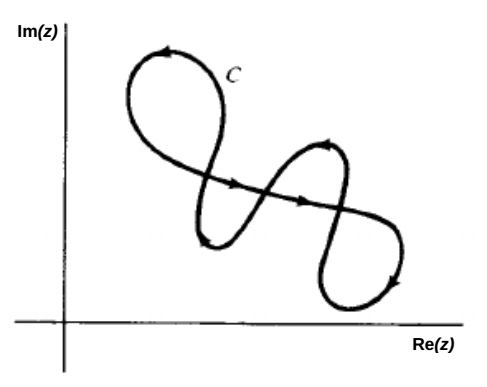
\includegraphics[scale=0.5]{curva_no_simple.png}
\end{center}

\end{multicols}

\colorbox{magenta!40!white!80}{\parbox{\linewidth}{
\theoremstyle{theorem}
\begin{theorem} {Teorema Integral de Cauchy-Goursat generalizado}

Si $f(z)$ es una funci\'on anal\'itica en un dominio $\mathcal{D}$ simplemente conexo, entonces para todo camino cerrado $\mathcal{C}$ contenido en $\mathcal{D}$: $$\oint\limits_{\mathcal{C}}f(z)\ dz = 0$$

\end{theorem}}}
\linebreak
\linebreak

Ahora la cuesti\'on es... cuando tienes una curva $\mathcal{C}$, definida como una curva cerrada suave pero en cuyo interior la funci\'on $f(z)$ no es anal\'itica para todo punto, ?`qu\'e hago? La soluci\'on a todos tus problemas viene dado por el siguiente teorema:\\

\colorbox{magenta!40!white!80}{\parbox{\linewidth}{
\theoremstyle{theorem}
\begin{theorem} {Teorema Integral de Cauchy para dominios m\'ultiplemente conexos}\\

Supongamos que:
\begin{itemize}
	\item Sea $\mathcal{C}$ una curva cerrada y simple, positivamente orientada.
	\item Sean $\mathcal{C}_k$ con $k=1,2,3.., n$ contornos cerrados simples, orientados positivamente, disjuntos y cuyos dominios interiores no tienen puntos en com\'un.
\end{itemize}

Si $f(z)$ es una funci\'on anal\'itica en todos estos contornos y en el dominio m\'ultiplemente conexo formado por todos los puntos interiores a $\mathcal{C}$ y exteriores a todos los $\mathcal{C}_k$, entonces $$\oint_{\mathcal{C}}f(z)\ dz = \sum\limits_{k=1}^n \left( \oint_{\mathcal{C}_k} f(z)\ dz \right)$$

\end{theorem}}}
\linebreak

Demostrar\\

Consideramos a los primeros teoremas enunciados en esta secci\'on como \textit{teoremas integrales para dominios simplemente conexos}. Y si tratamos con dominios m\'ultiplemente conexos, aplicamos el teorema reci\'en visto.\\

Una consecuencia importante del teorema anterior es el \textbf{Principio de la Deformaci\'on}.\\

\colorbox{pink!40!white!80}{\parbox{\linewidth}{
\theoremstyle{theorem}
\begin{corolary} {Principio de Deformaci\'on}

Sean $\mathcal{C}_1$ y $\mathcal{C}_2$ contornos cerrados simples orientados positivamente, donde $\mathcal{C}_2$ es interior a $\mathcal{C}_1$. Si una funci\'on $f(z)$ es anal\'itica en ambos caminos y en los puntos comprendidos entre ellos, entonces: $$\oint\limits_{\mathcal{C}_1}f(z)\ dz = \oint\limits_{\mathcal{C}_2}f(z)\ dz$$

\end{corolary}}}
\linebreak
\linebreak

Recapitulando, podemos resumir un poco lo visto hasta aqu\'i respecto de integrales de contorno, y exponer estas \textit{condiciones equivalentes} a la hora de analizar funciones de variable compleja.\\

\colorbox{magenta!40!white!80}{\parbox{\linewidth}{
\theoremstyle{theorem}
\begin{theorem} {Condiciones equivalentes}

Sea $f(z)$ una funci\'on continua en un dominio $\mathcal{D}$. Entonces las siguientes propiedades son equivalentes entre s\'i:
\begin{enumerate}
	\item $f(z)$ tiene una primitiva $F(z)$ en $\mathcal{D}$
	\item Las integrales de $f(z)$ sobre caminos contenidos en $\mathcal{D}$, con punto inicial $z_1$ y punto final $z_0$ fijos, tienen todas el mismo valor (independencia del camino)
	\item Las integrales de $f(z)$ sobre caminos cerrados contenidos en $\mathcal{D}$ tienen todas el mismo valor (cero).
\end{enumerate}

\end{theorem}}}
\linebreak
\linebreak

\begin{center}
	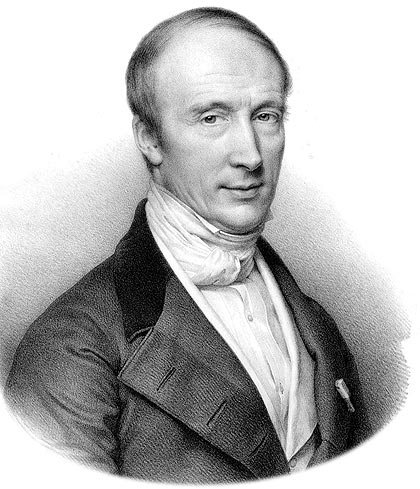
\includegraphics[scale=0.8]{cauchy.jpg}\\
	\textit{Augustin Louis Cauchy}
\end{center}

\subsection{F\'ormula Integral de Cauchy}
Como si no fuese suficente con tantos teoremas de Cauchy, veremos unas formulaciones m\'as, que son de suma importancia en el estudio de funciones de variable compleja.\\

\colorbox{red!40!white!80}{\parbox{\linewidth}{
\theoremstyle{theorem}
\begin{theorem} {F\'ormula Integral de Cauchy}

Sea $f(z)$  una funci\'on anal\'itica en un dominio $\mathcal{D}$. Sea $\mathcal{C}$ un contorno cerrado simple orientado positivamente en $\mathcal{D}$ que encierra \'unicamente puntos de $\mathcal{D}$. Si $z_0$ es un punto del dominio interior a $\mathcal{C}$, entonces: $$f(z_0) = \frac{1}{2\pi i}\oint\limits_{\mathcal{C}}\frac{f(z)}{z-z_0}\ dz$$

\end{theorem}}}
\linebreak

Demostrar\\

Bas\'andose en la f\'ormula del teorema anterior, llegamos a nuevas formas de calcular la derivada de tales funciones...\\

\colorbox{pink!40!white!80}{\parbox{\linewidth}{
\theoremstyle{theorem}
\begin{corolary} {F\'ormula Integral: extensi\'on a derivadas de orden superior}\\

Sea $f(z)$  una funci\'on anal\'itica en un dominio $\mathcal{D}$. Sea $\mathcal{C}$ un contorno cerrado simple orientado positivamente en $\mathcal{D}$ que encierra \'unicamente puntos de $\mathcal{D}$. Si $z$ es un punto del dominio interior a $\mathcal{C}$, entonces:
$$f'(z) = \frac{1}{2\pi i}\oint\limits_{\mathcal{C}}\frac{f(s)}{(s-z)^2}\ ds \qquad f''(z) = \frac{1}{\pi i}\oint\limits_{\mathcal{C}}\frac{f(s)}{(s-z)^3}\ ds$$

Tenemos de forma gen\'erica que: $$f^{(n)}(z) = \frac{n!}{2\pi i}\oint\limits_{\mathcal{C}}\frac{f(s)}{(s-z)^{n+1}}\ ds$$

\end{corolary}}}
\linebreak
\linebreak

A esta altura, contamos con las herramientas necesarias para poder demostrar un teorema que se expuso hace un tiempo en \textsf{Derivaci\'on Compleja}. Es el de analiticidad de las derivadas, que a continuaci\'on lo exponemos por mayor comodidad, y redactado en nuevos t\'erminos.\\

\colorbox{red!40!white!80}{\parbox{\linewidth}{
\theoremstyle{theorem}
\begin{theorem} {Analiticidad de las derivadas}

Sea $f(z)$  una funci\'on anal\'itica en un dominio $\mathcal{D}$. Sea $\mathcal{C}$ un contorno cerrado simple orientado positivamente en $\mathcal{D}$ que encierra \'unicamente puntos de $\mathcal{D}$.

Si $z$ es un punto del dominio interior a $\mathcal{C}$, entonces $f(z)$ tiene derivadas de todos los \'ordenes en ese punto y son anal\'iticas en \'el.

\end{theorem}}}
\linebreak

Demostrar\\


\end{document}